\section{PI Table reduction and Petrick's method}
This is not in the text-book. For additional reading, please refer to the linked resources on the website.
\\

\includegraphics[width=0.7\linewidth]{1952-quine.png}\\
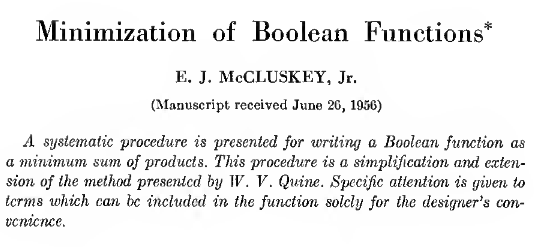
\includegraphics[width=0.7\linewidth]{1956-mccluskey.png}


\begin{definition}[Implicant]
  Given a function $f$ of $n$ variables, a product term $P$ is an implicant of $f$
  if and only if for every combination of values of the $n$ variables for which $P=1$, $f$ is
  also equal to 1.
\end{definition}

\begin{definition}[Prime Implicant]
  A prime implicant of a function $f$ is an implicant which is no longer an
  implicant if any literal is removed from it.
\end{definition}

There are 4 main steps in the Quine-McCluskey algorithm/PI Table reduction and Petrick's method:

\begin{enumerate}
\item Generate Prime Implicants
\item Construct Prime Implicant Table. PIs as columns, and minterms as
  rows (don't cares are excluded).
\item Reduce Prime Implicant Table by repeating following steps until they
  it cannot be reduced further
\begin{enumerate}
  \item Remove Essential Prime Implicants
  \item Row Dominance: Remove \emph{dominating} rows. (i.e. unnecessary minterms)
  \item Column Dominance: Remove \emph{dominated} columns. (i.e. remove unnecessary PIs)
\end{enumerate}
\item Solve Prime Implicant Table by Petrick's method
\end{enumerate}


\subsection{Generate Prime Implicants}

\begin{example}
  Generate prime implicants of the function 
  \[ F (A, B, C, D) = \sum m(0, 2, 4, 6, 7,
  8, 10, 12, 13, 14, 16, 18, 19, 29, 30)\]
  using Quine-McCluskey method
\end{example}
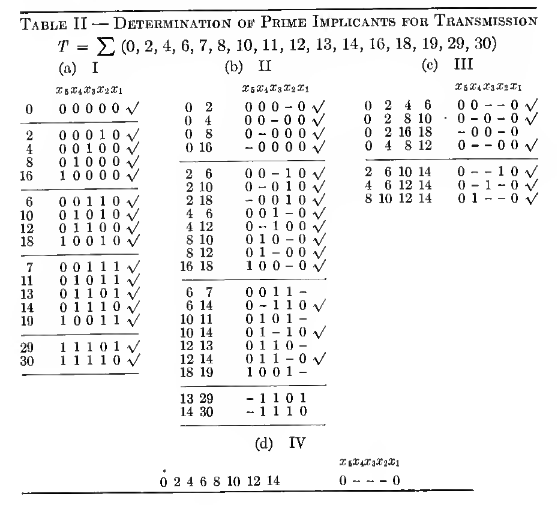
\includegraphics[width=0.9\linewidth]{1956-mccluskey-table-2.png}

Steps:
\begin{enumerate}
  \item Start with writing minterms in binary format (include don't cares as minterms).
  \item Create potential groups of minterms that can be combined (merged). The only
    minterms that can be combined differ only be single 1. Create a new list of
    combined minterms as n-1 literal implicants.
  \item Check off the minterms that could be combined. Unchecked minterms are
    prime implicants (PIs).
  \item Repeat the grouping process with n-1 literal implicants.
\end{enumerate}

% \begin{prob}
%   Generate PIs for the function $ F(A, B, C, D) = \sum m(0, 2, 3, 4, 5, 6, 7, 8,
%   9, 10, 11, 12, 13)$.
% \end{prob}

\subsection{Prime Implicants table and reduction}

\begin{example}
  Reduce the prime implicants $\{ \bB \bD, C\bD, BD, BC, A\bD, AB \}$ using prime
  implicants table.
\end{example}
\vspace{20em}

\begin{example}
  \begin{Karnaugh}{AB}{CD}
    \minterms{0,4,5,13,15,11}
    \maxterms{1,2,3,6,7,8,9,10,12,14}
    \implicant{0}{4}{red}
    \implicant{4}{5}{blue}
    \implicant{5}{13}{green}
    \implicant{13}{15}{cyan}
    \implicant{15}{11}{orange}
  \end{Karnaugh}
\end{example}
\vspace{10em}

\begin{example}
  \begin{Karnaugh}{AB}{CD}
    \minterms{1,2,3,5,7}
    \indeterminants{0,6,9,13}
    \maxterms{4,8,10,11,12,14,15}
    \implicant{0}{2}{red}
    \implicant{1}{7}{blue}
    \implicant{1}{6}{green}
    \implicant{1}{9}{cyan}
  \end{Karnaugh}
\end{example}
\vspace{10em}

\begin{example}
  Reduce the following PI table\\
  \begin{tabular}{r|ccccccccc}
    \toprule
    & $\bA\bD$ & $\bB\bD$ & $\bC\bD$ & $\bA C$ & $\bB C$ & $\bA B$ & $B \bC$& $A\bB$ & $A \bC$ \\
    \midrule
     0 & X & X & X &   &   &   &   &   &   \\
     2 & X & X &   & X & X &   &   &   &   \\
     3 &   &   &   & X & X &   &   &   &   \\
     4 & X &   & X &   &   & X & X &   &   \\
     5 &   &   &   &   &   & X & X &   &   \\
     6 & X &   &   & X &   & X &   &   &   \\
     7 &   &   &   & X &   & X &   &   &   \\
     8 &   & X & X &   &   &   &   & X & X \\
     9 &   &   &   &   &   &   &   & X & X \\
    10 &   & X &   &   & X &   &   & X &   \\
    11 &   &   &   &   & X &   &   & X &   \\
    12 &   &   & X &   & X &   & X &   & X \\
    13 &   &   &   &   &   &   & X &   & X \\
    \bottomrule
  \end{tabular}
\end{example}
\vspace{20em}
\begin{example}
  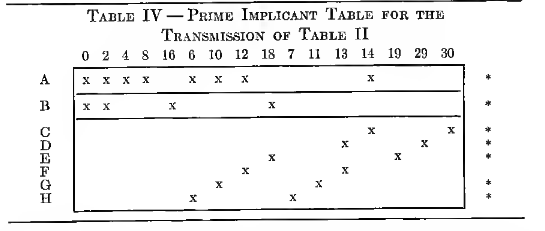
\includegraphics[width=\linewidth]{1956-mccluskey-table-4.png}
\end{example}

\subsection{Petrick's method}

\begin{example}
  Solve the Prime Implicant table using Petrick's method\\
  \begin{tabular}{r|cccccc}
    \toprule
    & $p_1 = \bA C$ & $p_2 = \bB C$ & $p_3 = \bA B$ & $p_4 = B \bC$& $p_5 = A\bB$ & $p_6 = A \bC$ \\
    \midrule
     3 & X & X &   &   &   &   \\
     5 &   &   & X & X &   &   \\
     7 & X &   & X &   &   &   \\
     9 &   &   &   &   & X & X \\
    11 &   & X &   &   & X &   \\
    13 &   &   &   & X &   & X \\
    \bottomrule
  \end{tabular}
\end{example}
\vspace{20em}


% \begin{example}
%   Find the minimum SOP expression for the function $F (A, B, C, D) = \sum m(2, 3, 7,
%   9, 11, 13) + \sum d(1, 10, 15)$ using Quine-McCluskey method.
% \end{example}
